One of the main reasons we selected the Play! Framework is because this framework has been proven in production. For example the LinkedIn web application has been developed using the Play! Framework. The following figure\ref{play} illustrates an overview of the Play! Framework.\\
\begin{figure}[h!]
\centering
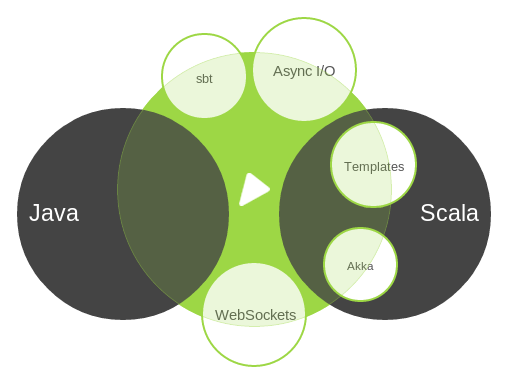
\includegraphics[scale=0.5]{./img/play.png}
\caption{\small{The main attributes and features of the Play! Framework}}
\label{play}
\end{figure}
 
 
The Play! Framework offers excellent documentation\cite{playDoc} that can help us get familiar with the Play! environment. First of all, it is an open source application that has an amazing error handling because of the fact that everything is compiled and built on the fly. This makes it easier for developers to detect bugs and can dramatically improve the developer's productivity to make changes. By reloading the browser, you can immediately see the changes you just made, which makes it perfect for fast prototyping within our project. Moreover, Play! supports both the Scala and Java languages, it comes with a Scala template that allows you to write dynamic code within an HTML body, and it also comes with pre-configured testing support. This last one is particularly important because that means we do not need to worry about adding Junit dependencies to the build file. \\\\
Play! also offers the use of the EBean server interface which is very handy for fetching and saving beans to a particular DataSource. It can make reactive applications simpler because Play! is built on \href{http://netty.io/}{Netty}, which means it supports non-blocking I/O.\footnote{ non-blocking I/O is a form of input/output processing that permits other processing to continue before the transmission has finished.} This will enable our web application to make remote calls inexpensively which is crucial for high performance web applications.

\newpage




